\section{Experiments}
\label{sec:experiments}

\subsection{Setup}

We fine-tune two decoder-only models, at 1.4B and 7B parameters, on a 2.1M
example instruction pool assembled from eight public sources. Four target
benchmarks supply the shift: \textsc{LegalQA-S} (statutory question answering
against a pool with almost no legal text), \textsc{BioSum} (abstractive
summarisation of clinical trial abstracts), \textsc{FinNER} (entity extraction
from filings), and \textsc{CodeDoc} (docstring generation for a private
codebase). Each benchmark contributes 256 anchor examples and a disjoint test
split of at least 2{,}000 examples. The token budget is fixed at 180M tokens
for every method, which is 8.6 percent of the pool.

Baselines are uniform random sampling; top-loss selection, which keeps the
examples with the highest current loss; gradient-norm selection following
\citet{arbogast2021gradnorm}; embedding-space nearest neighbour retrieval
against the anchor set~\citep{iwasaki2022retrieval}; and facility-location
submodular selection~\citep{delacroix2020submodular}. We also report full-pool
fine-tuning at 2.1B tokens as an upper reference. Every configuration is run
with three seeds and we report the mean.

\subsection{Main results}

Table~\ref{tab:main} gives target accuracy at the fixed budget. \method{} is
the best selection method on all four benchmarks at both scales, and at 7B it
recovers full-pool accuracy while reading 31 percent of the tokens that the
full-pool run consumes. The gap to the second-best method is widest on
\textsc{LegalQA-S}, the benchmark whose target domain is least represented in
the pool, which is what an anchored criterion should predict.

\begin{table}[t]
  \centering
  \small
  \caption{Target accuracy (percent) at a fixed 180M token budget, mean over
  three seeds. Full-pool fine-tuning consumes 2.1B tokens and is shown for
  reference rather than as a competitor. Best selection method in bold.}
  \label{tab:main}
  \begin{tabular}{llrrrrr}
    \toprule
    Scale & Method & \textsc{LegalQA-S} & \textsc{BioSum} & \textsc{FinNER}
          & \textsc{CodeDoc} & Avg. \\
    \midrule
    \multirow{6}{*}{1.4B}
      & Random                & 41.2 & 33.8 & 62.4 & 48.1 & 46.4 \\
      & Top loss              & 39.7 & 34.6 & 61.0 & 47.3 & 45.7 \\
      & Gradient norm         & 42.8 & 35.1 & 63.7 & 49.6 & 47.8 \\
      & Nearest neighbour     & 45.9 & 36.0 & 64.2 & 51.4 & 49.4 \\
      & Facility location     & 46.3 & 36.4 & 64.9 & 51.0 & 49.7 \\
      & \textbf{\method{}}    & \textbf{50.1} & \textbf{38.2} & \textbf{66.8}
                              & \textbf{53.7} & \textbf{52.2} \\
    \midrule
    \multirow{6}{*}{7B}
      & Random                & 52.6 & 41.9 & 71.8 & 60.2 & 56.6 \\
      & Top loss              & 51.4 & 42.5 & 70.9 & 59.5 & 56.1 \\
      & Gradient norm         & 54.0 & 43.1 & 72.6 & 61.4 & 57.8 \\
      & Nearest neighbour     & 57.2 & 44.0 & 73.1 & 63.0 & 59.3 \\
      & Facility location     & 57.8 & 44.6 & 73.6 & 62.7 & 59.7 \\
      & \textbf{\method{}}    & \textbf{62.4} & \textbf{46.8} & \textbf{75.9}
                              & \textbf{65.8} & \textbf{62.7} \\
    \midrule
    7B & Full pool (2.1B tokens) & 62.9 & 47.1 & 76.2 & 66.0 & 63.1 \\
    \bottomrule
  \end{tabular}
\end{table}

Top-loss selection is below random at both scales. Inspecting its selections
explains why: 22 percent of the examples it keeps at the 1.4B scale are
truncated or mislabelled records that the pool's own filters missed. High loss
identifies them reliably and they teach the model nothing.

\subsection{Budget efficiency}

Figure~\ref{fig:curves} plots target accuracy against consumed tokens on
\textsc{LegalQA-S} at 7B. The anchored curriculum's advantage appears early and
narrows late, which is the behaviour the temperature schedule is designed to
produce: once $\tau_t$ approaches 1 the sampling distribution is nearly uniform
and \method{} is spending its remaining budget much as random selection would.

\begin{figure}[t]
  \centering
  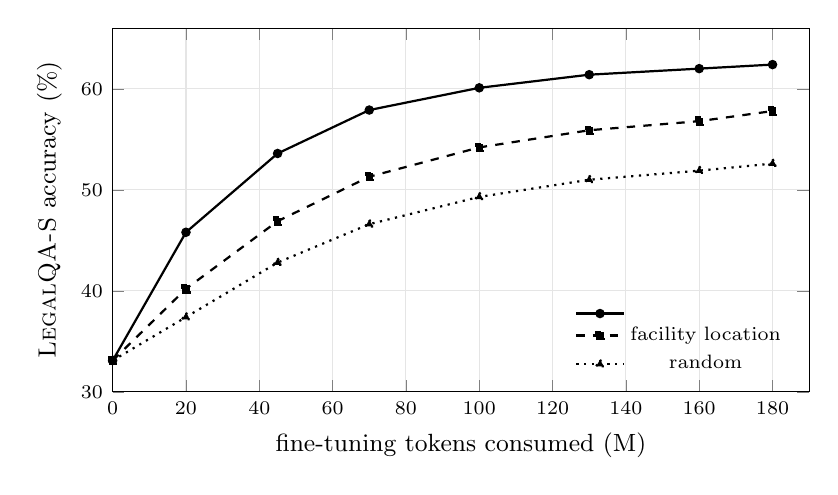
\begin{tikzpicture}
    \begin{axis}[
        width=0.86\linewidth, height=6.2cm,
        xlabel={fine-tuning tokens consumed (M)},
        ylabel={\textsc{LegalQA-S} accuracy (\%)},
        xmin=0, xmax=190, ymin=30, ymax=66,
        grid=both, grid style={gray!20},
        legend style={font=\scriptsize,at={(0.98,0.02)},anchor=south east,
                      draw=none,fill=none},
        tick label style={font=\scriptsize},
        label style={font=\small},
      ]
      \addplot[thick,mark=*,mark size=1.3pt] coordinates {
        (0,33.1) (20,45.8) (45,53.6) (70,57.9) (100,60.1)
        (130,61.4) (160,62.0) (180,62.4)
      };
      \addlegendentry{\method{}}
      \addplot[thick,dashed,mark=square*,mark size=1.3pt] coordinates {
        (0,33.1) (20,40.2) (45,46.9) (70,51.3) (100,54.2)
        (130,55.9) (160,56.8) (180,57.8)
      };
      \addlegendentry{facility location}
      \addplot[thick,dotted,mark=triangle*,mark size=1.6pt] coordinates {
        (0,33.1) (20,37.4) (45,42.8) (70,46.6) (100,49.3)
        (130,51.0) (160,51.9) (180,52.6)
      };
      \addlegendentry{random}
    \end{axis}
  \end{tikzpicture}
  \caption{Accuracy against consumed budget on \textsc{LegalQA-S} at 7B.
  \method{} passes the final accuracy of random selection after 56M tokens,
  roughly a third of the budget.}
  \label{fig:curves}
\end{figure}
